\documentclass[12pt,oneside,a4paper,chapter=TITLE,section=TITLE,english]{abntex2}
\usepackage[T1]{fontenc}
\usepackage[utf8]{inputenc}
\usepackage{amsmath,amssymb}
\usepackage{graphicx}
\usepackage{booktabs}
\usepackage{microtype}
\usepackage{float}
\usepackage[alf]{abntex2cite}
% Notação de unidades sem dependência do pacote siunitx.
\newcommand{\SI}[2]{#1\,#2}
\newcommand{\hertz}{\ensuremath{\mathrm{Hz}}}
\newcommand{\radian}{\ensuremath{\mathrm{rad}}}
\newcommand{\second}{\ensuremath{\mathrm{s}}}
\newcommand{\milli}{\ensuremath{\mathrm{m}}}
\newcommand{\per}{\ensuremath{\,/\,}}
\setlength{\emergencystretch}{2em}
\renewcommand{\ABNTEXchapterfontsize}{\large}
\renewcommand{\ABNTEXsectionfontsize}{\normalsize}
\renewcommand{\ABNTEXchapterfont}{\rmfamily}
\setlength{\beforechapskip}{2\baselineskip}
\setlength{\afterchapskip}{1.0\baselineskip}
\hypersetup{hidelinks}
\def\clearforchapter{\relax}

\titulo{Projeto e comparação de filtros digitais IIR e FIR}
\autor{Ana Iara Loayza Costa\\José Victor Brito Costa\\Milena Freire Britto Neves}
\local{São Luís}
\data{2026}
\instituicao{Universidade Federal do Maranhão --- UFMA\\Centro de Ciências Exatas e Tecnologia\\Curso de Engenharia da Computação}
\tipotrabalho{Trabalho acadêmico}
\preambulo{Trabalho referente à 3ª Avaliação da disciplina EECP0018 --- Processamento Digital de Sinais, sob orientação do Prof. Dr. Pedro Baptista Fernandes.}

\begin{document}
\frenchspacing
\renewcommand{\contentsname}{Sumário}
\renewcommand{\bibname}{Referências}
\pretextual
\imprimircapa
\imprimirfolhaderosto

\begin{resumo}
Este trabalho projeta dois filtros digitais passa-baixas para remover componentes acima
de \SI{50}{\hertz} de um sinal composto por senoides de 10, 120 e \SI{200}{\hertz},
amostrado a \SI{500}{\hertz}. Primeiramente, projeta-se um Butterworth analógico de
terceira ordem. A transformação bilinear, com pré-distorção da frequência crítica,
produz um IIR digital com corte exato em \SI{50}{\hertz}. Em seguida, projeta-se um FIR
de ordem 40 pelo método da janela de Hamming. As respostas em frequência e ao impulso
são apresentadas, os dois filtros são aplicados ao sinal e suas características são
comparadas. O IIR alcança transição mais seletiva com poucos coeficientes, enquanto o
FIR oferece estabilidade inerente e fase exatamente linear.

\textbf{Palavras-chave}: filtros digitais; Butterworth; transformação bilinear; filtro FIR; janela de Hamming.
\end{resumo}

\pdfbookmark[0]{\contentsname}{toc}
\tableofcontents*
\textual

\newpage

\chapter{Introdução}
Filtros digitais permitem selecionar componentes espectrais por meio de algoritmos
executados sobre amostras. Neste trabalho são consideradas as duas famílias principais:
filtros com resposta ao impulso infinita (IIR) e filtros com resposta ao impulso finita
(FIR). O primeiro é obtido de um protótipo Butterworth analógico pela transformação
bilinear; o segundo, pelo truncamento de uma resposta ideal com uma janela de Hamming
\cite{oppenheim2013,proakis2007}. Todos os cálculos e simulações foram realizados em
Python, e todas as rotinas completas acompanham o relatório no notebook
\texttt{PDS\_ATV3.ipynb}.

\chapter{Geração e amostragem do sinal}
O sinal pedido é
\begin{equation}
x(t)=\sin(20\pi t)+0{,}6\sin(240\pi t)+0{,}3\sin(400\pi t).
\end{equation}
Comparando cada argumento com $2\pi f t$, suas frequências são
\begin{equation}
f_1=\frac{20\pi}{2\pi}=\SI{10}{\hertz},\quad
f_2=\frac{240\pi}{2\pi}=\SI{120}{\hertz},\quad
f_3=\frac{400\pi}{2\pi}=\SI{200}{\hertz}.
\end{equation}
Para $F_s=\SI{500}{\hertz}$, $T_s=1/F_s=\SI{2}{\milli\second}$ e um segundo de
observação produz 500 amostras, nos instantes $t_n=n/500$, $0\leq n\leq499$. Logo,
\begin{equation}
x[n]=\sin(0{,}04\pi n)+0{,}6\sin(0{,}48\pi n)+0{,}3\sin(0{,}8\pi n).
\end{equation}
Como $F_s/2=\SI{250}{\hertz}>f_{\max}=\SI{200}{\hertz}$, não ocorre sobreposição
espectral por subamostragem \cite{haykin2001}. A Figura~\ref{fig:sinal} sobrepõe a
curva contínua e as amostras.
\begin{figure}[H]\centering
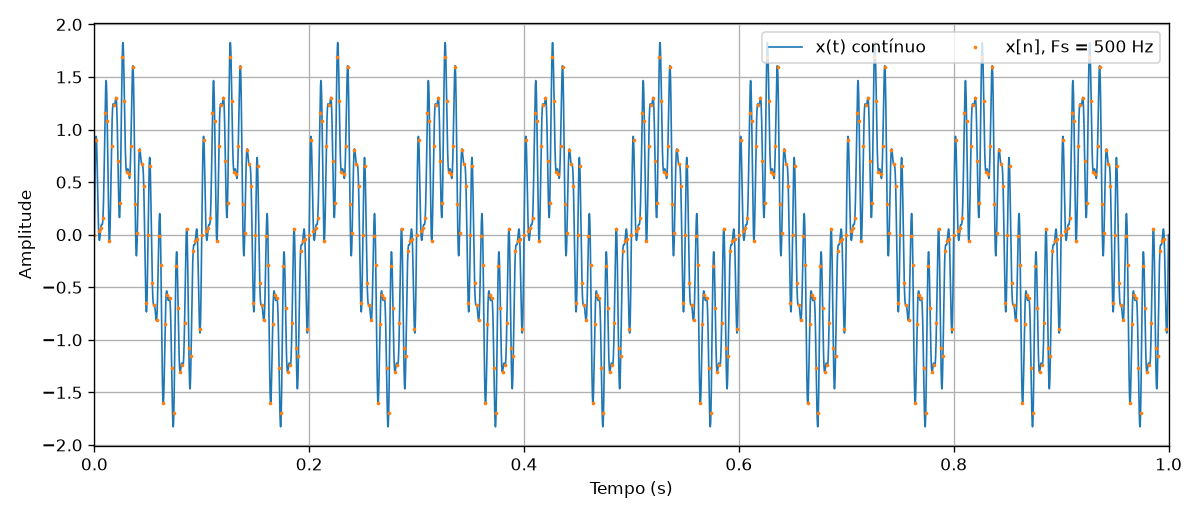
\includegraphics[width=\textwidth]{images/sinal_continuo_amostrado.png}
\caption{Sinal contínuo durante um segundo e sinal amostrado a \SI{500}{\hertz}.}\label{fig:sinal}
\end{figure}

\chapter{Filtro Butterworth analógico}
\section{Função de transferência}
Deseja-se preservar a componente de \SI{10}{\hertz} e atenuar as componentes acima de
\SI{50}{\hertz}. O protótipo Butterworth normalizado de ordem 3 tem polos em
$-1$ e $-1/2\pm j\sqrt{3}/2$, portanto
\begin{equation}
H_N(s)=\frac{1}{(s+1)(s^2+s+1)}=\frac{1}{s^3+2s^2+2s+1}.
\end{equation}
Com $\Omega_c=2\pi(50)=\SI{314.1593}{\radian\per\second}$ e a transformação de escala
$s\mapsto s/\Omega_c$, obtém-se
\begin{equation}\label{eq:ha}
H_a(s)=\frac{\Omega_c^3}{s^3+2\Omega_cs^2+2\Omega_c^2s+\Omega_c^3}.
\end{equation}
Numericamente,
\begin{equation}
H_a(s)=\frac{3{,}10063\times10^7}{s^3+628{,}3185s^2+1{,}97392\times10^5s+3{,}10063\times10^7}.
\end{equation}
O Butterworth é maximamente plano na banda passante e satisfaz
\begin{equation}
|H_a(j\Omega)|=\frac{1}{\sqrt{1+(\Omega/\Omega_c)^6}}.
\end{equation}
Assim, em $\Omega=\Omega_c$, $|H_a|=1/\sqrt2$ ou $-3{,}0103$ dB.

\section{Diagrama de Bode}
A Figura~\ref{fig:bode} identifica o corte. Após a região de transição, a ordem 3
resulta em inclinação assintótica de $-60$ dB/década.
\begin{figure}[H]\centering
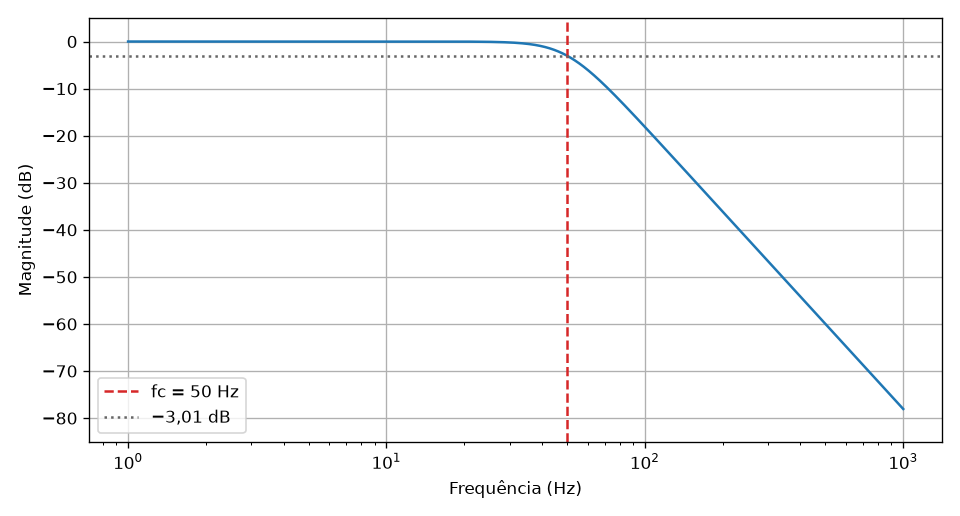
\includegraphics[width=.86\textwidth]{images/bode_analogico.png}
\caption{Diagrama de Bode de magnitude do Butterworth analógico.}\label{fig:bode}
\end{figure}

\chapter{Filtro digital IIR por transformação bilinear}
\section{Especificações e dedução}
As especificações são: passa-baixas Butterworth, ordem 3, $F_s=\SI{500}{\hertz}$,
$f_c=\SI{50}{\hertz}$ e ganho unitário em corrente contínua. A transformação bilinear
é
\begin{equation}\label{eq:bilinear}
s=2F_s\frac{1-z^{-1}}{1+z^{-1}}.
\end{equation}
Ela mapeia todo o eixo $j\Omega$ no círculo unitário sem aliasing e preserva a
estabilidade, mas deforma a frequência segundo
\begin{equation}
\Omega=2F_s\tan\!\left(\pi\frac{f}{F_s}\right).
\end{equation}
Usar diretamente $\Omega_c=2\pi50$ deslocaria o corte digital para
$f=(F_s/\pi)\arctan(\Omega_c/2F_s)=\SI{48.45}{\hertz}$. Portanto, para obter exatamente
\SI{50}{\hertz}, aplica-se a pré-distorção
\begin{equation}
\Omega_p=2(500)\tan(\pi 50/500)=\SI{324.9197}{\radian\per\second}.
\end{equation}
Substituindo $\Omega_p$ na Equação~\eqref{eq:ha} e depois a
Equação~\eqref{eq:bilinear}, chega-se a
\begin{equation}\label{eq:iir}
H_{IIR}(z)=\frac{0{,}01809893+0{,}05429680z^{-1}+0{,}05429680z^{-2}+0{,}01809893z^{-3}}
{1-1{,}76004188z^{-1}+1{,}18289326z^{-2}-0{,}27805992z^{-3}}.
\end{equation}
Os polos têm módulos menores que 1 (o maior é aproximadamente $0{,}739$), logo o
filtro causal é BIBO-estável.

\section{Respostas em frequência e ao impulso}
A resposta em frequência é obtida avaliando a Equação~\eqref{eq:iir} em
$z=e^{j2\pi f/F_s}$. Ela aparece na Figura~\ref{fig:freq}, junto ao FIR para facilitar
a comparação. A resposta ao impulso da Figura~\ref{fig:impulso} é infinita, embora
decresça por causa da estabilidade dos polos.

\chapter{Filtro FIR por janela de Hamming}
\section{Especificações e coeficientes}
O segundo projeto é passa-baixas, $F_s=\SI{500}{\hertz}$, $f_c=\SI{50}{\hertz}$,
ordem $N=40$ (41 coeficientes), janela de Hamming e fase linear. A frequência digital
é $\omega_c=2\pi f_c/F_s=0{,}2\pi$. Centralizando a resposta ideal em $N/2=20$,
\begin{equation}
h_d[n]=\frac{\sin[\omega_c(n-20)]}{\pi(n-20)}
=\frac{2f_c}{F_s}\,\operatorname{sinc}\!\left[\frac{2f_c}{F_s}(n-20)\right],
\end{equation}
com o valor limite $h_d[20]=2f_c/F_s=0{,}2$. A janela é
\begin{equation}
w[n]=0{,}54-0{,}46\cos\left(\frac{2\pi n}{40}\right),\quad0\leq n\leq40,
\end{equation}
e os coeficientes finais são $h[n]=h_d[n]w[n]$, normalizados por
$\sum_{n=0}^{40}h[n]$ para tornar $H(1)=1$. Como $h[n]=h[40-n]$, a fase é linear e o
atraso de grupo é exatamente $N/2=20$ amostras, ou \SI{40}{\milli\second}.

\section{Respostas}
\begin{figure}[H]\centering
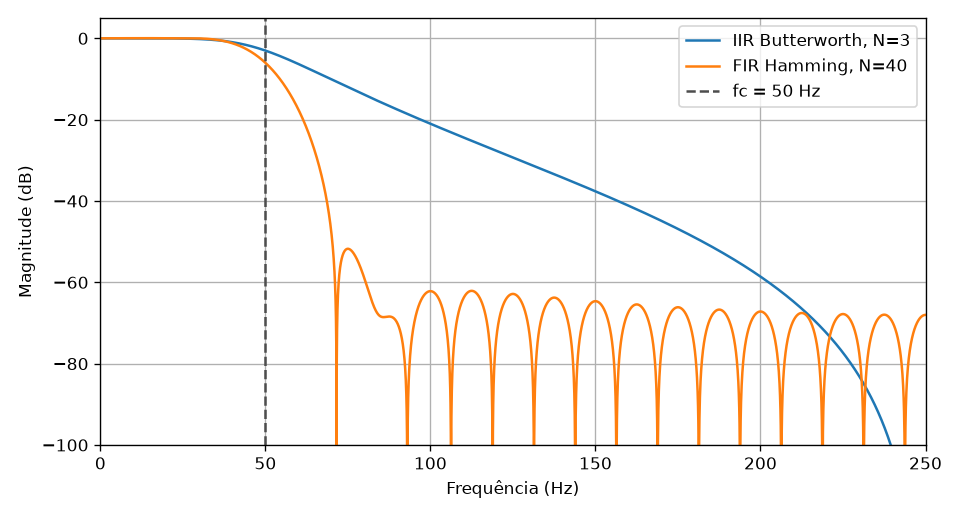
\includegraphics[width=.9\textwidth]{images/respostas_frequencia.png}
\caption{Respostas em frequência dos filtros digitais e corte especificado.}\label{fig:freq}
\end{figure}
\begin{figure}[H]\centering
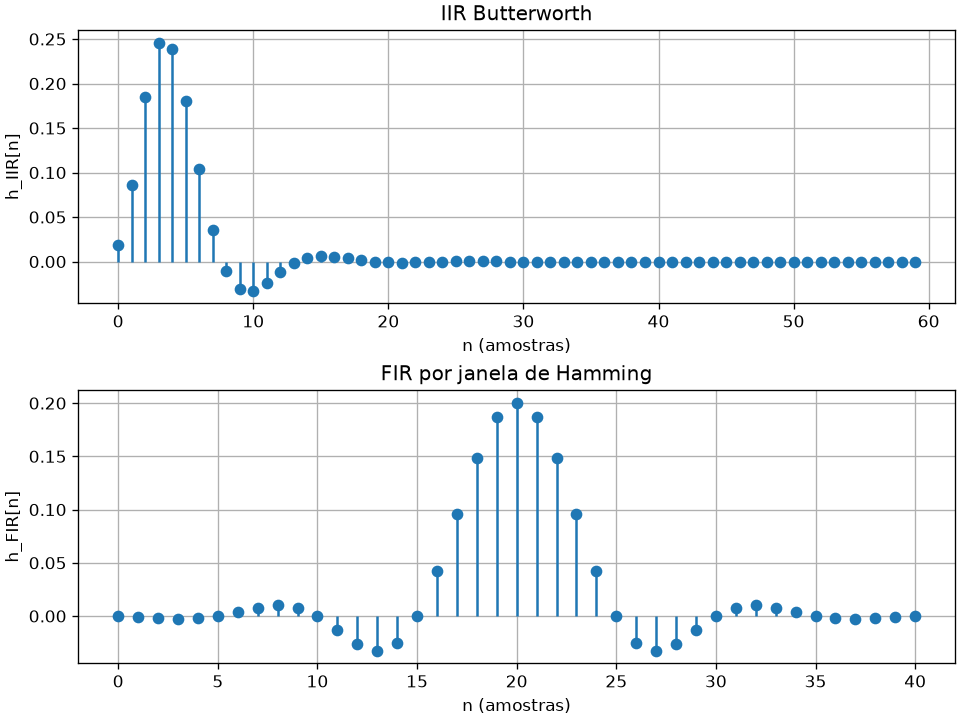
\includegraphics[width=.88\textwidth]{images/respostas_impulso.png}
\caption{Respostas ao impulso: IIR infinita e FIR com 41 amostras.}\label{fig:impulso}
\end{figure}

\chapter{Aplicação dos filtros ao sinal}
Para ambos os filtros, a saída foi calculada diretamente pela equação de diferenças
\begin{equation}
y[n]=\sum_{k=0}^{M}b_kx[n-k]-\sum_{k=1}^{N}a_ky[n-k],\qquad a_0=1.
\end{equation}
No FIR, $a_k=0$ para $k>0$. A Figura~\ref{fig:saidas} mantém os sinais na escala de
tempo causal: o deslocamento visível do FIR corresponde ao seu atraso de grupo de
20 amostras. Após os transitórios, ambos preservam essencialmente a senoide de
\SI{10}{\hertz} e rejeitam as oscilações de 120 e \SI{200}{\hertz}.
\begin{figure}[H]\centering
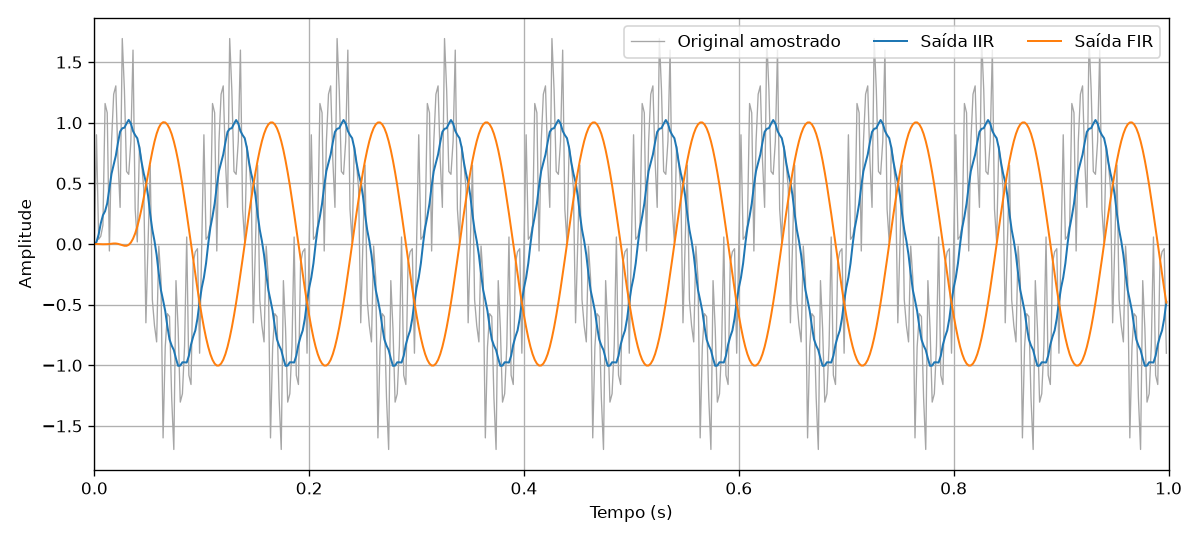
\includegraphics[width=\textwidth]{images/comparacao_saidas.png}
\caption{Sinal amostrado e saídas causais dos filtros IIR e FIR.}\label{fig:saidas}
\end{figure}

\chapter{Comparação objetiva}
\section{Vantagens e desvantagens}
\begin{table}[H]\centering
\caption{Comparação entre as estruturas projetadas}
\begin{tabular}{@{}p{2.4cm}p{5.4cm}p{5.4cm}@{}}\toprule
&\textbf{IIR Butterworth}&\textbf{FIR Hamming}\\\midrule
Vantagens&Transição seletiva com ordem baixa; apenas quatro coeficientes no numerador e quatro no denominador; menor custo e memória.&Estabilidade inerente; fase exatamente linear; ausência de realimentação; menor sensibilidade à quantização.\\
Desvantagens&Fase não linear; realimentação e maior sensibilidade numérica; pode tornar-se instável com projeto ou quantização inadequados.&41 multiplicações por amostra; maior memória; atraso fixo de 20 amostras; transição mais larga para a ordem escolhida.\\\bottomrule
\end{tabular}
\end{table}

\section{Indicação para tempo real}
Para uma aplicação em tempo real com recursos computacionais limitados e sem exigência
de fase linear, o \textbf{IIR de terceira ordem é o mais indicado}: cumpre a filtragem
com muito menos operações e menor latência. Se a forma de onda ou o alinhamento
temporal das componentes for crítico, o FIR passa a ser preferível por sua fase linear
e robustez, aceitando-se o custo e a latência adicionais. Portanto, ``tempo real'' não
determina sozinho a família; neste problema, a solução IIR é a escolha mais econômica.

\chapter{Conclusão}
Os seis itens do projeto foram atendidos. O sinal foi corretamente amostrado sem
aliasing; o Butterworth analógico de ordem 3 foi deduzido e convertido em um IIR
estável com corte digital corrigido por pré-distorção; e o FIR de ordem 40 foi obtido
pela janela de Hamming. As simulações confirmaram a remoção das componentes acima de
\SI{50}{\hertz}. A comparação evidencia o compromisso fundamental: eficiência e baixa
latência no IIR contra fase linear e robustez no FIR.

\postextual
\bibliography{referencias}
\end{document}
